% mnras_template.tex
%
% LaTeX template for creating an MNRAS paper
%
% v3.0 released 14 May 2015
% (version numbers match those of mnras.cls)
%
% Copyright (C) Royal Astronomical Society 2015
% Authors:
% Keith T. Smith (Royal Astronomical Society)

% Change log
%
% v3.0 May 2015
%    Renamed to match the new package name
%    Version number matches mnras.cls
%    A few minor tweaks to wording
% v1.0 September 2013
%    Beta testing only - never publicly released
%    First version: a simple (ish) template for creating an MNRAS paper

%%%%%%%%%%%%%%%%%%%%%%%%%%%%%%%%%%%%%%%%%%%%%%%%%%
% Basic setup. Most papers should leave these options alone.
\documentclass[a4paper,fleqn,usenatbib]{mnras}

% MNRAS is set in Times font. If you don't have this installed (most LaTeX
% installations will be fine) or prefer the old Computer Modern fonts, comment
% out the following line
\usepackage{newtxtext,newtxmath}
% Depending on your LaTeX fonts installation, you might get better results with one of these:
%\usepackage{mathptmx}
%\usepackage{txfonts}

% Use vector fonts, so it zooms properly in on-screen viewing software
% Don't change these lines unless you know what you are doing
\usepackage[T1]{fontenc}
\usepackage{ae,aecompl}


%%%%% AUTHORS - PLACE YOUR OWN PACKAGES HERE %%%%%
% \usepackage(graphicx,tabularx}

% Only include extra packages if you really need them. Common packages are:
\usepackage{graphicx}	% Including figure files
\usepackage{amsmath}	% Advanced maths commands
\usepackage{amssymb}	% Extra maths symbols

%%%%%%%%%%%%%%%%%%%%%%%%%%%%%%%%%%%%%%%%%%%%%%%%%%

%%%%% AUTHORS - PLACE YOUR OWN COMMANDS HERE %%%%%

% Please keep new commands to a minimum, and use \newcommand not \def to avoid
% overwriting existing commands. Example:
%\newcommand{\pcm}{\,cm$^{-2}$}	% per cm-squared

%%%%%%%%%%%%%%%%%%%%%%%%%%%%%%%%%%%%%%%%%%%%%%%%%%

%%%%%%%%%%%%%%%%%%% TITLE PAGE %%%%%%%%%%%%%%%%%%%

% Title of the paper, and the short title which is used in the headers.
% Keep the title short and informative.
\title[CSS081231]{CSS081231: A short period eclipsing polar}

% The list of authors, and the short list which is used in the headers.
% If you need two or more lines of authors, add an extra line using \newauthor
\author[R.P. Ashley et al.]{
R.P. Ashley,$^{1}$\thanks{E-mail: r.p.ashley@warwick.ac.uk}
A. Aungwerojwit,$^{2, 3}$
B.T. G{\"a}nsicke$^{1}$
M.A. Hollands$^{1}$
and T.R. Marsh$^{1}$
\\
% List of institutions
$^{1}$Department of Physics, University of Warwick, Gibbet Hill Road, Coventry, CV4 7AL, UK\\
$^{2}$Department of Physics, Faculty of Science, Naresuan University, Phitsanulok 65000, Thailand\\
$^{3}$ThEP Center, CHE, 328 Si Ayutthaya Road, Bangkok 10400, Thailand
}

% These dates will be filled out by the publisher
\date{Accepted XXX. Received YYY; in original form ZZZ}

% Enter the current year, for the copyright statements etc.
\pubyear{2015}

% Don't change these lines
\begin{document}
\label{firstpage}
\pagerange{\pageref{firstpage}--\pageref{lastpage}}
\maketitle

% Abstract of the paper
\begin{abstract}
CSS081231:071126+440405 is an eclipsing polar with a period of 117 minutes. Small and medium sized telescopes have photometry of the system dating back to late 2008. The ephemeris was computed shortly after discovery and then revised recently following five years of subsequent observations. Newer photometric observations have allowed us to place tighter contraints on the orbital parameters. We have obtained six optical spectra of the system covering phases 0.24 to 0.90 during outburst and sixteen optical spectra taken during quiescence. The spectra show clear cyclotron humps, revealing magnetic field strength of $B  \sim 34 MG$.
\end{abstract}

% Select between one and six entries from the list of approved keywords.
% Don't make up new ones.
\begin{keywords}
stars -- individual -- CSS081231:071126+440405 -- binares: eclipsing -- stars: cataclysmic variables
\end{keywords}

%%%%%%%%%%%%%%%%%%%%%%%%%%%%%%%%%%%%%%%%%%%%%%%%%%

%%%%%%%%%%%%%%%%% BODY OF PAPER %%%%%%%%%%%%%%%%%%

\section{Introduction}

This is a simple template for authors to write new MNRAS papers.
See \texttt{mnras\_sample.tex} for a more complex example, and \texttt{mnras\_guide.tex}
for a full user guide.

All papers should start with an Introduction section, which sets the work
in context, cites relevant earlier studies in the field by \citet{Others2013},
and describes the problem the authors aim to solve \citep[e.g.][]{Author2012}.

CSS081231:071126+440405 is not a ROSAT source, but it appears in the Swift X-Ray Telescope Point Source Catalog \citep{2014ApJS..210....8E}. It was detected at $3.36 ^{+0.83} _{-0.72} cts/s$ in the full 0.3-10keV band, but the fluxes for the individual soft, medium and hard bands are also given. It is available from Vizier as catalogue IX/43.


\section{Observations}
Six nights of photometry were obtained using ULTRASPEC \citep{ULTRASPEC}, mounted on the 2.5m Thai National Telescope during 2014 and 2015. Exposure times varied from 1.6 to 3.6 seconds depending on the conditions of the night. For the first three observations the Sloane g filter was used and for the last three observations the KG5 filter was used. The KG5 filter has a broad optical passband stretching from $\sim3500 \AA~ \mbox{to} \sim7000 \AA$ and was chosen to allow the maximum light throughput without any potential contamination in the red from the M dwarf companion.  Data was reduced using the ULTRACAM pipeline (Marsh reference) with a comparison star located about xx arcminutes to XX from the target and located at RA, DEC. The details for these nights is shown in table \ref{tab:photometry}. 

\begin{table}
  \caption{Photometry used in this study. The instrument used was ULTRASPEC, mounted on the 2.5m Thai National Telescope at the Thai National Observatory.}
  \begin{tabular}{ l  l  l  l  l  }
  \hline
  Instrument & Date & Filter & $T_{\mbox{exp}}$& Total time \\
  \hline
    TNT - ULTRASPEC & 2014/02/06 & Sloan g (tbc)& 1.6s & 147.8m \\
    TNT - ULTRASPEC & 2014/02/07 & Sloan g (tbc)& 1.7s & 166.2m \\
    TNT - ULTRASPEC & 2014/02/08 & Sloan g (tbc)& 2.8s & 73.6m \\
    TNT - ULTRASPEC & 2014/12/12 & KG5 & 3.6s & 95.1m \\
    TNT - ULTRASPEC & 2015/01/01 & KG5 & 2.0s & 118.2m \\
    TNT - ULTRASPEC & 2015/01/03 & KG5 & 2.0s & 131.1m \\
    
  \hline
  \end{tabular}
  \label{tab:photometry}
\end{table}

The ephemeris given by \citet{Schwope2015} is 
\begin{equation}BJD(TDB) = 2454833.207868(14) + E\times0.0813768094(6)\end{equation}
but since our observations have been taken with instruments operating at a much higher time resolution than the sources used by Schwope, we have re-computed the ephemeris by combining our own eclipse times with those documented in the Schwope paper. Our recomputed ephemeris is 
\begin{equation}BJD(TDB) = 2454833.207854(12) + E\times0.0813768096(5)\end{equation}
a revised O-C plot is shown in Fig. \ref{fig:ocdiagram} with the new eclipse times are indicated in green. The light curve for all of our high time resolution photometry is shown in Fig. \ref{fig:lightcurves}.

% O-C Diagram
\begin{figure}
	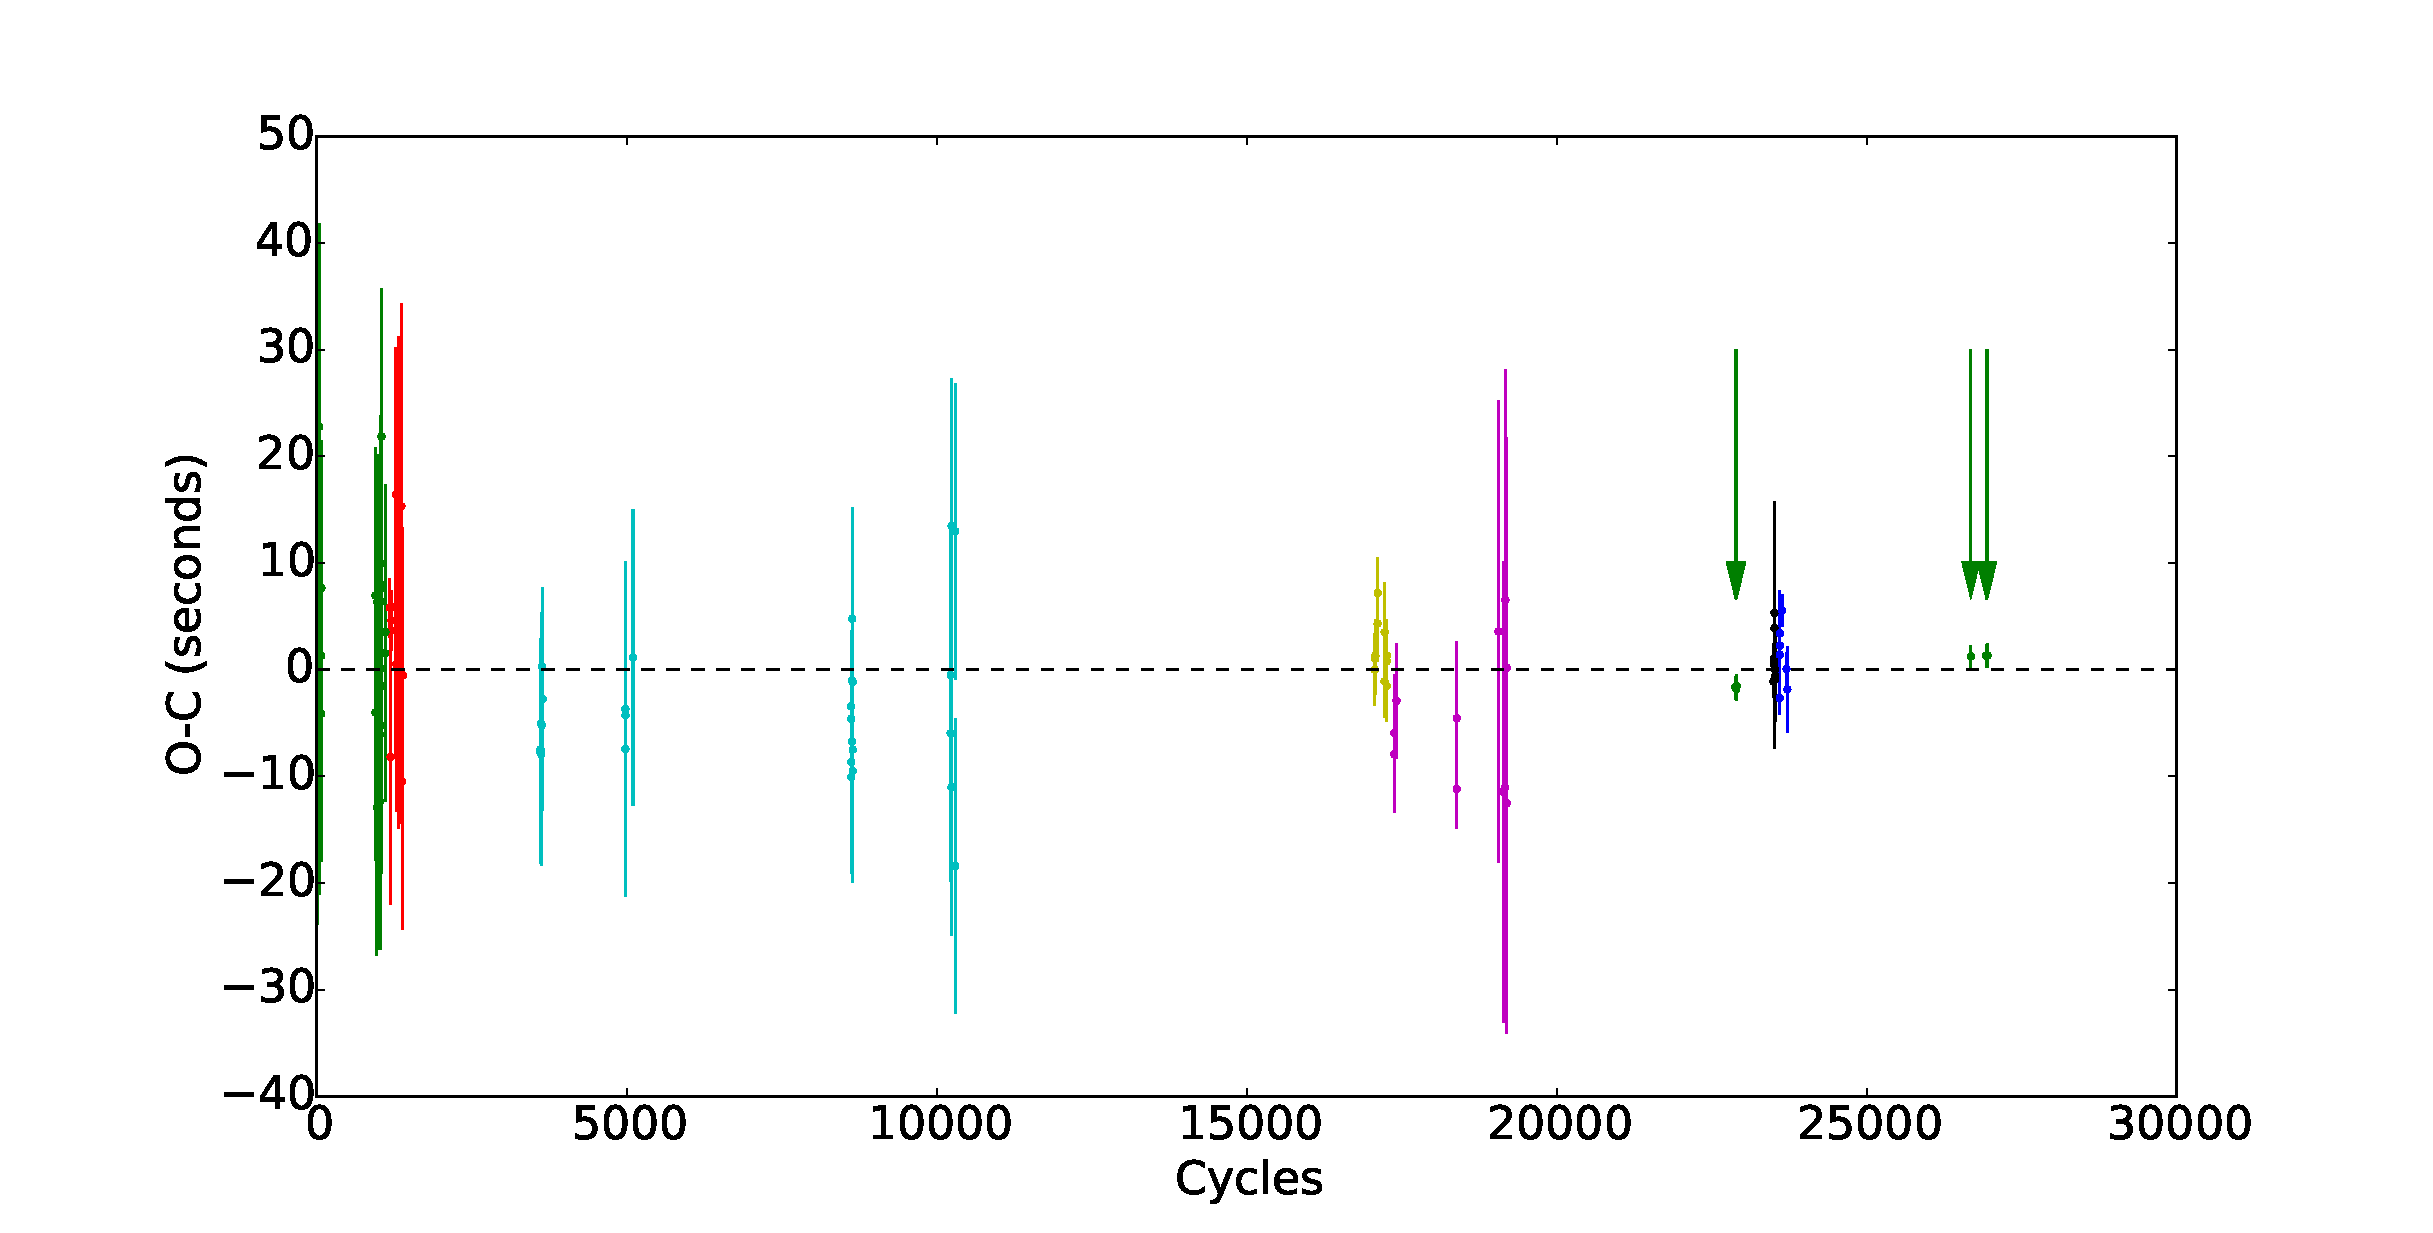
\includegraphics[width=\columnwidth]{images/css081231_oc.eps}
    \caption{The observed minus calculated times for all of the eclipse data as reported by \citet{Schwope2015} with our additional observations shown in green (on the right of the plot). }
    \label{fig:ocdiagram}
\end{figure}

% TNT light curves.
\begin{figure*}
\centering
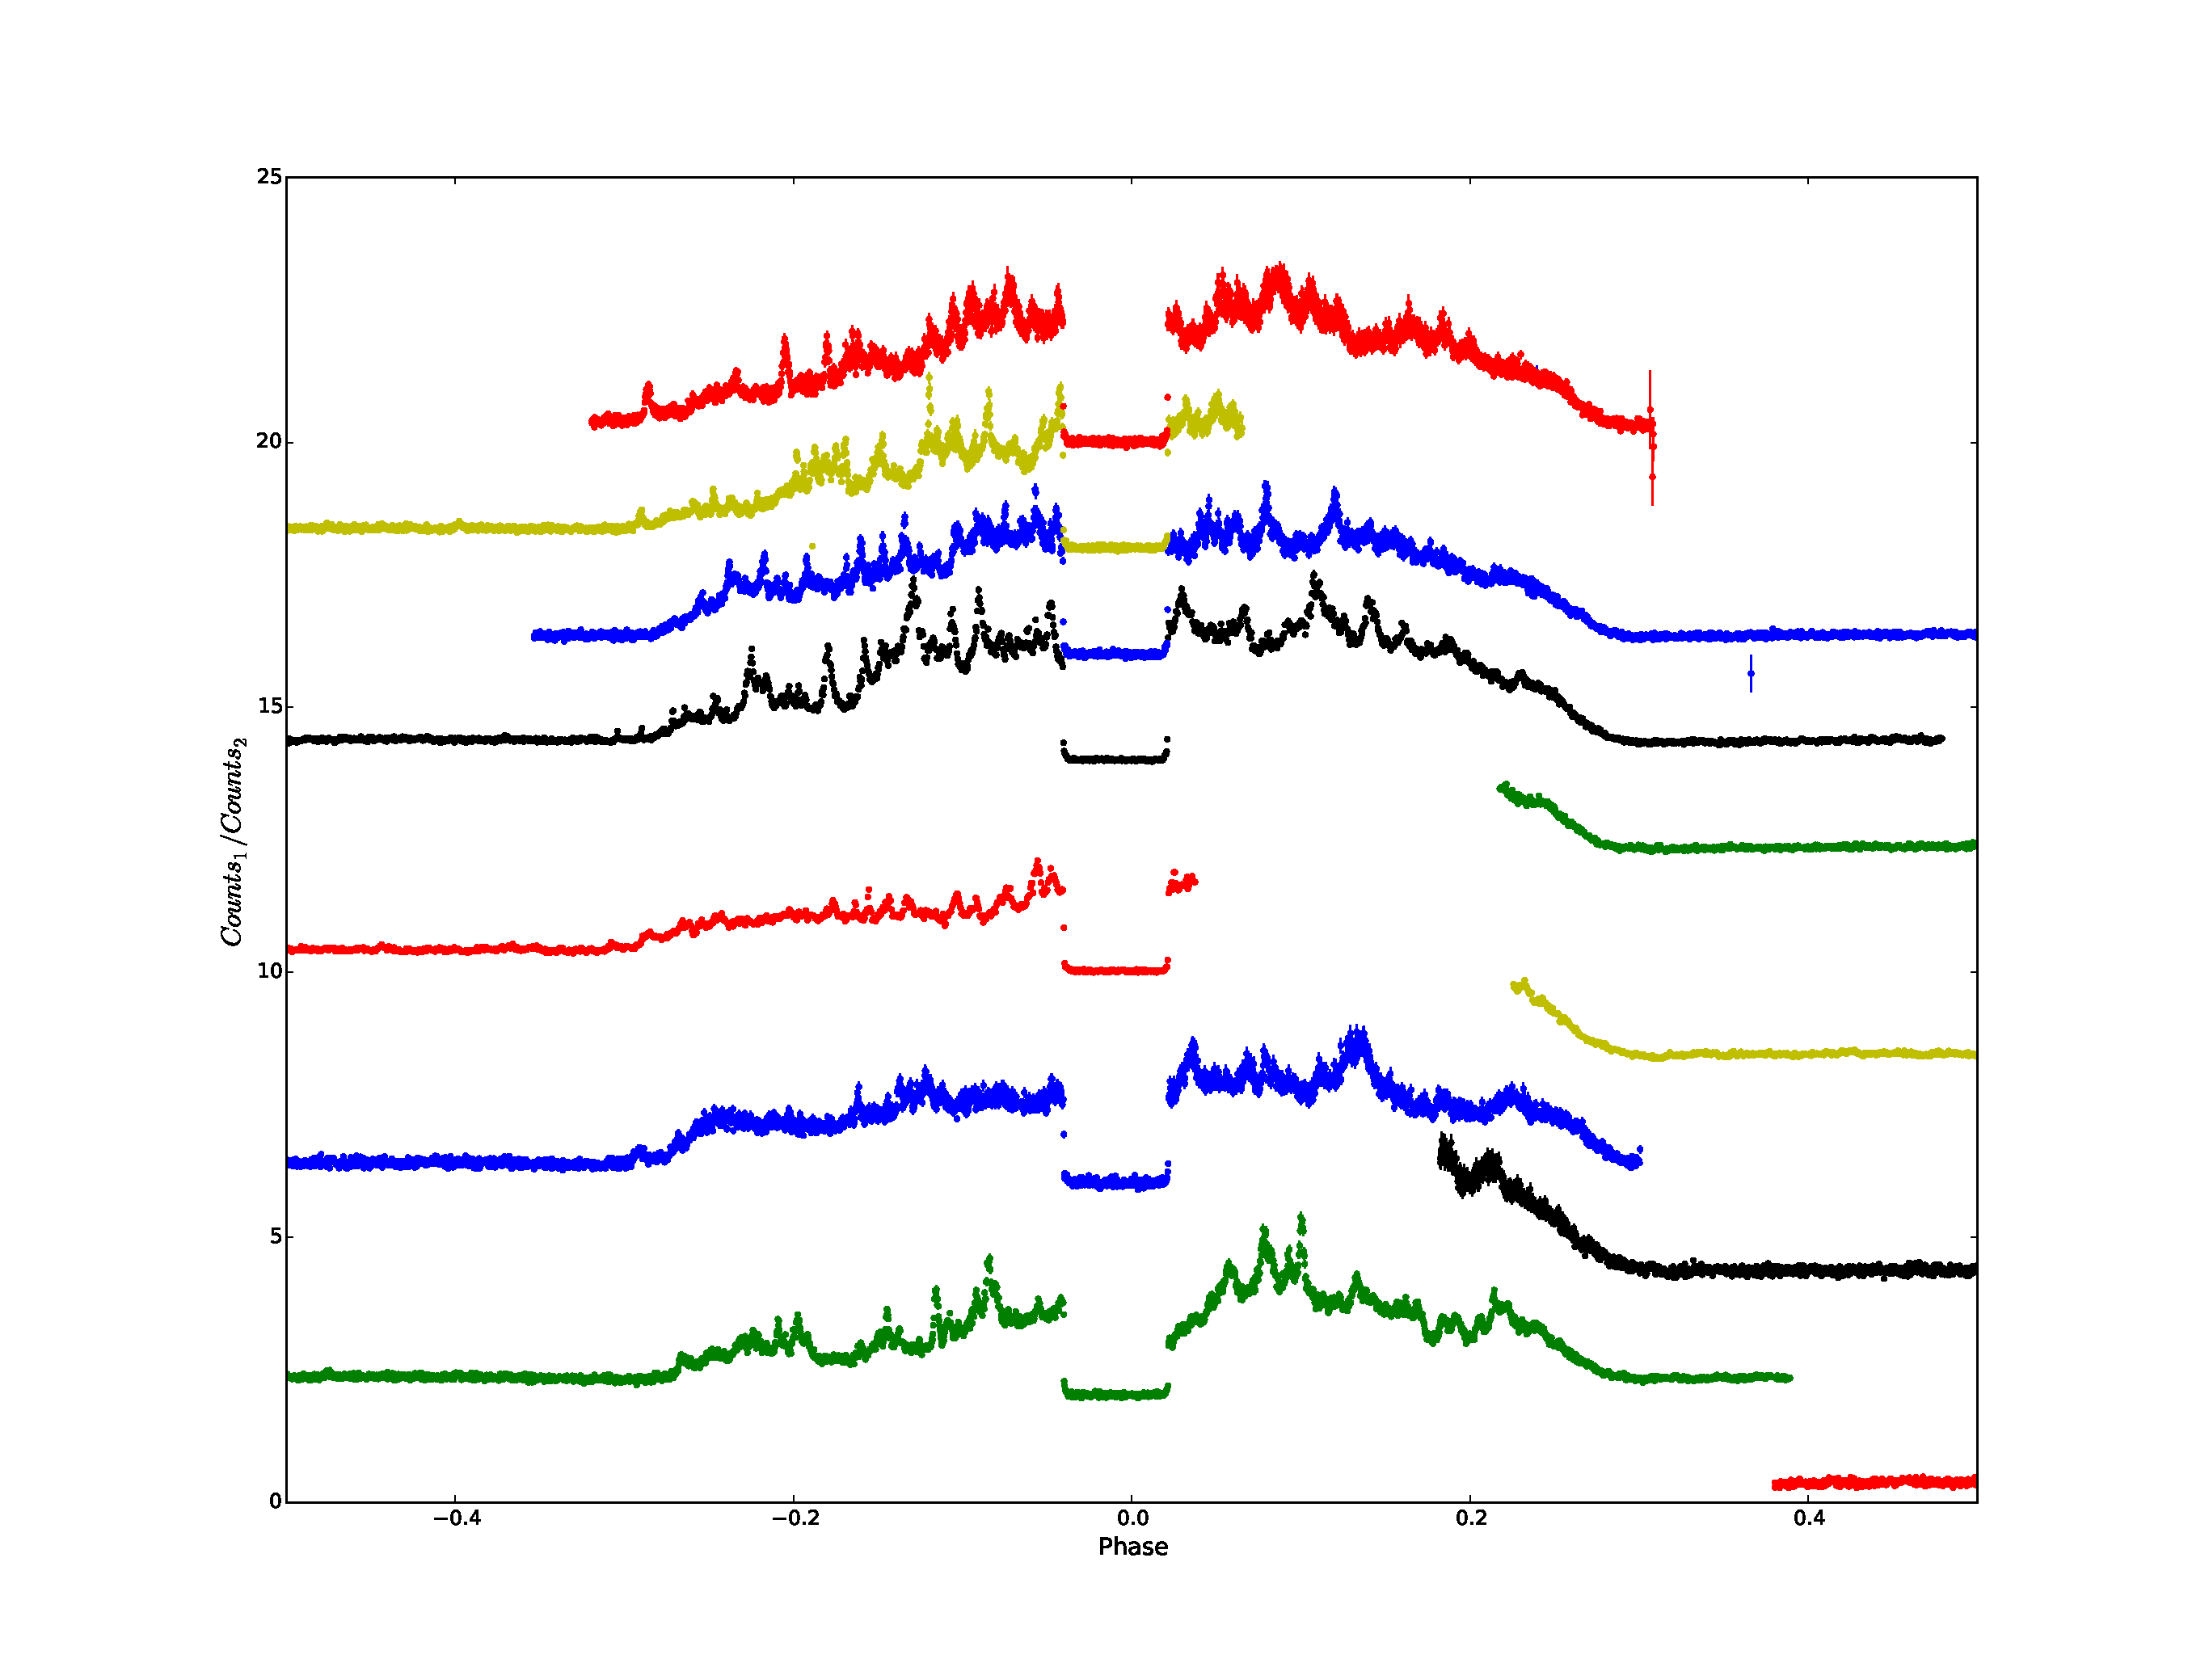
\includegraphics[width=\textwidth]{images/CSS081231_TNT_photometry.eps}
\caption[Caption for photometry]{The light curves of CSS081231. Exposure lengths vary from 1.6 to 3.6 seconds. The brightness of our target is measured as the fractional counts relative to our comparison star (described in the text). Each orbit is offset by 2 units for clarity.}
\label{fig:lightcurves}
\end{figure*}

% Radial velocity fit
\begin{figure}
\centering
\includegraphics[height=\columnwidth, angle=270]{images/NaIrvfit.eps}
\caption[Caption for RVs]{A fit to the computed radial velocities of the Na I doublet at 8183\AA~ and 8194\AA. The $K_2$ amplitude for the fit is 435(12) km/s.     }
\label{fig:rv-fit}
\end{figure}

% Outburst spectra
\begin{figure*}
\centering
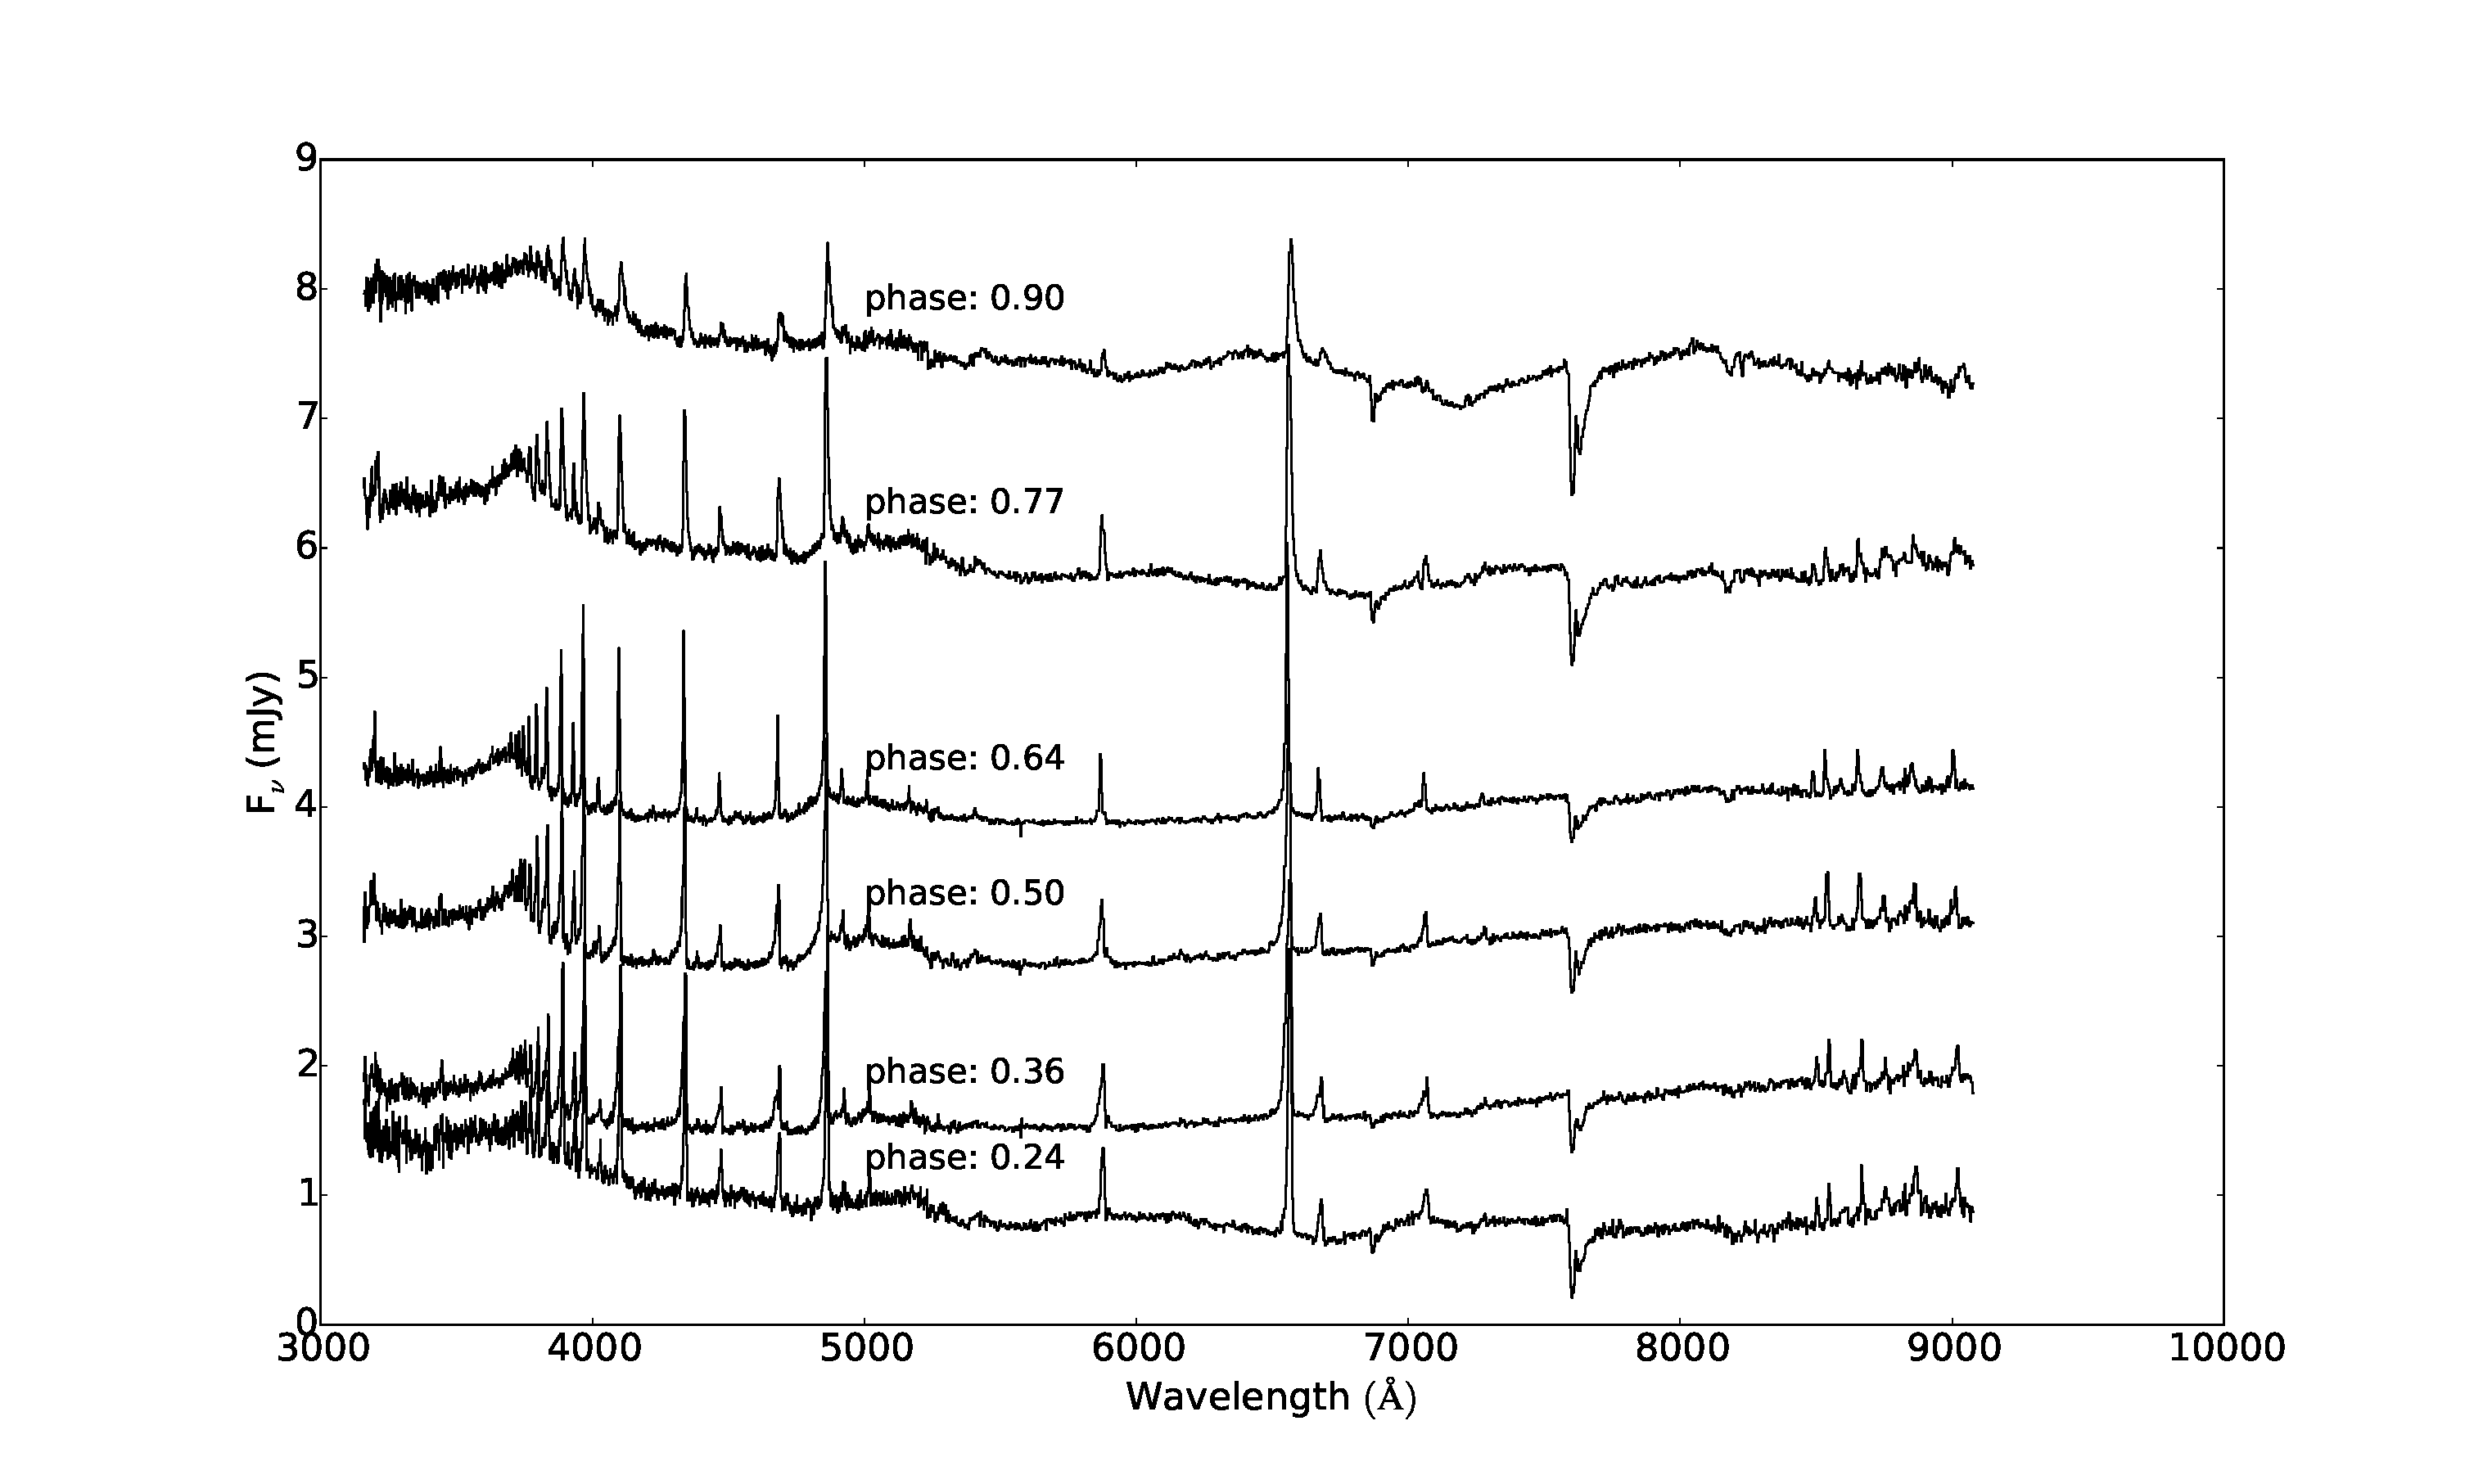
\includegraphics[width=\textwidth]{images/CSS081231_spectra.eps}
\caption[Caption for spectra]{The optical spectra of CSS081231 taken at 6 stages of the orbital cycle during outburst in December 2014. Cyclotron humps are seen in the early and late stages of the orbit when the accretion spot is in view. During the mid-phases of the orbit the accretion spot is eclipsed by the white dwarf. }
\label{fig:spectra-outpurst}
\end{figure*}

% Quiescent spectra
\begin{figure*}
\centering
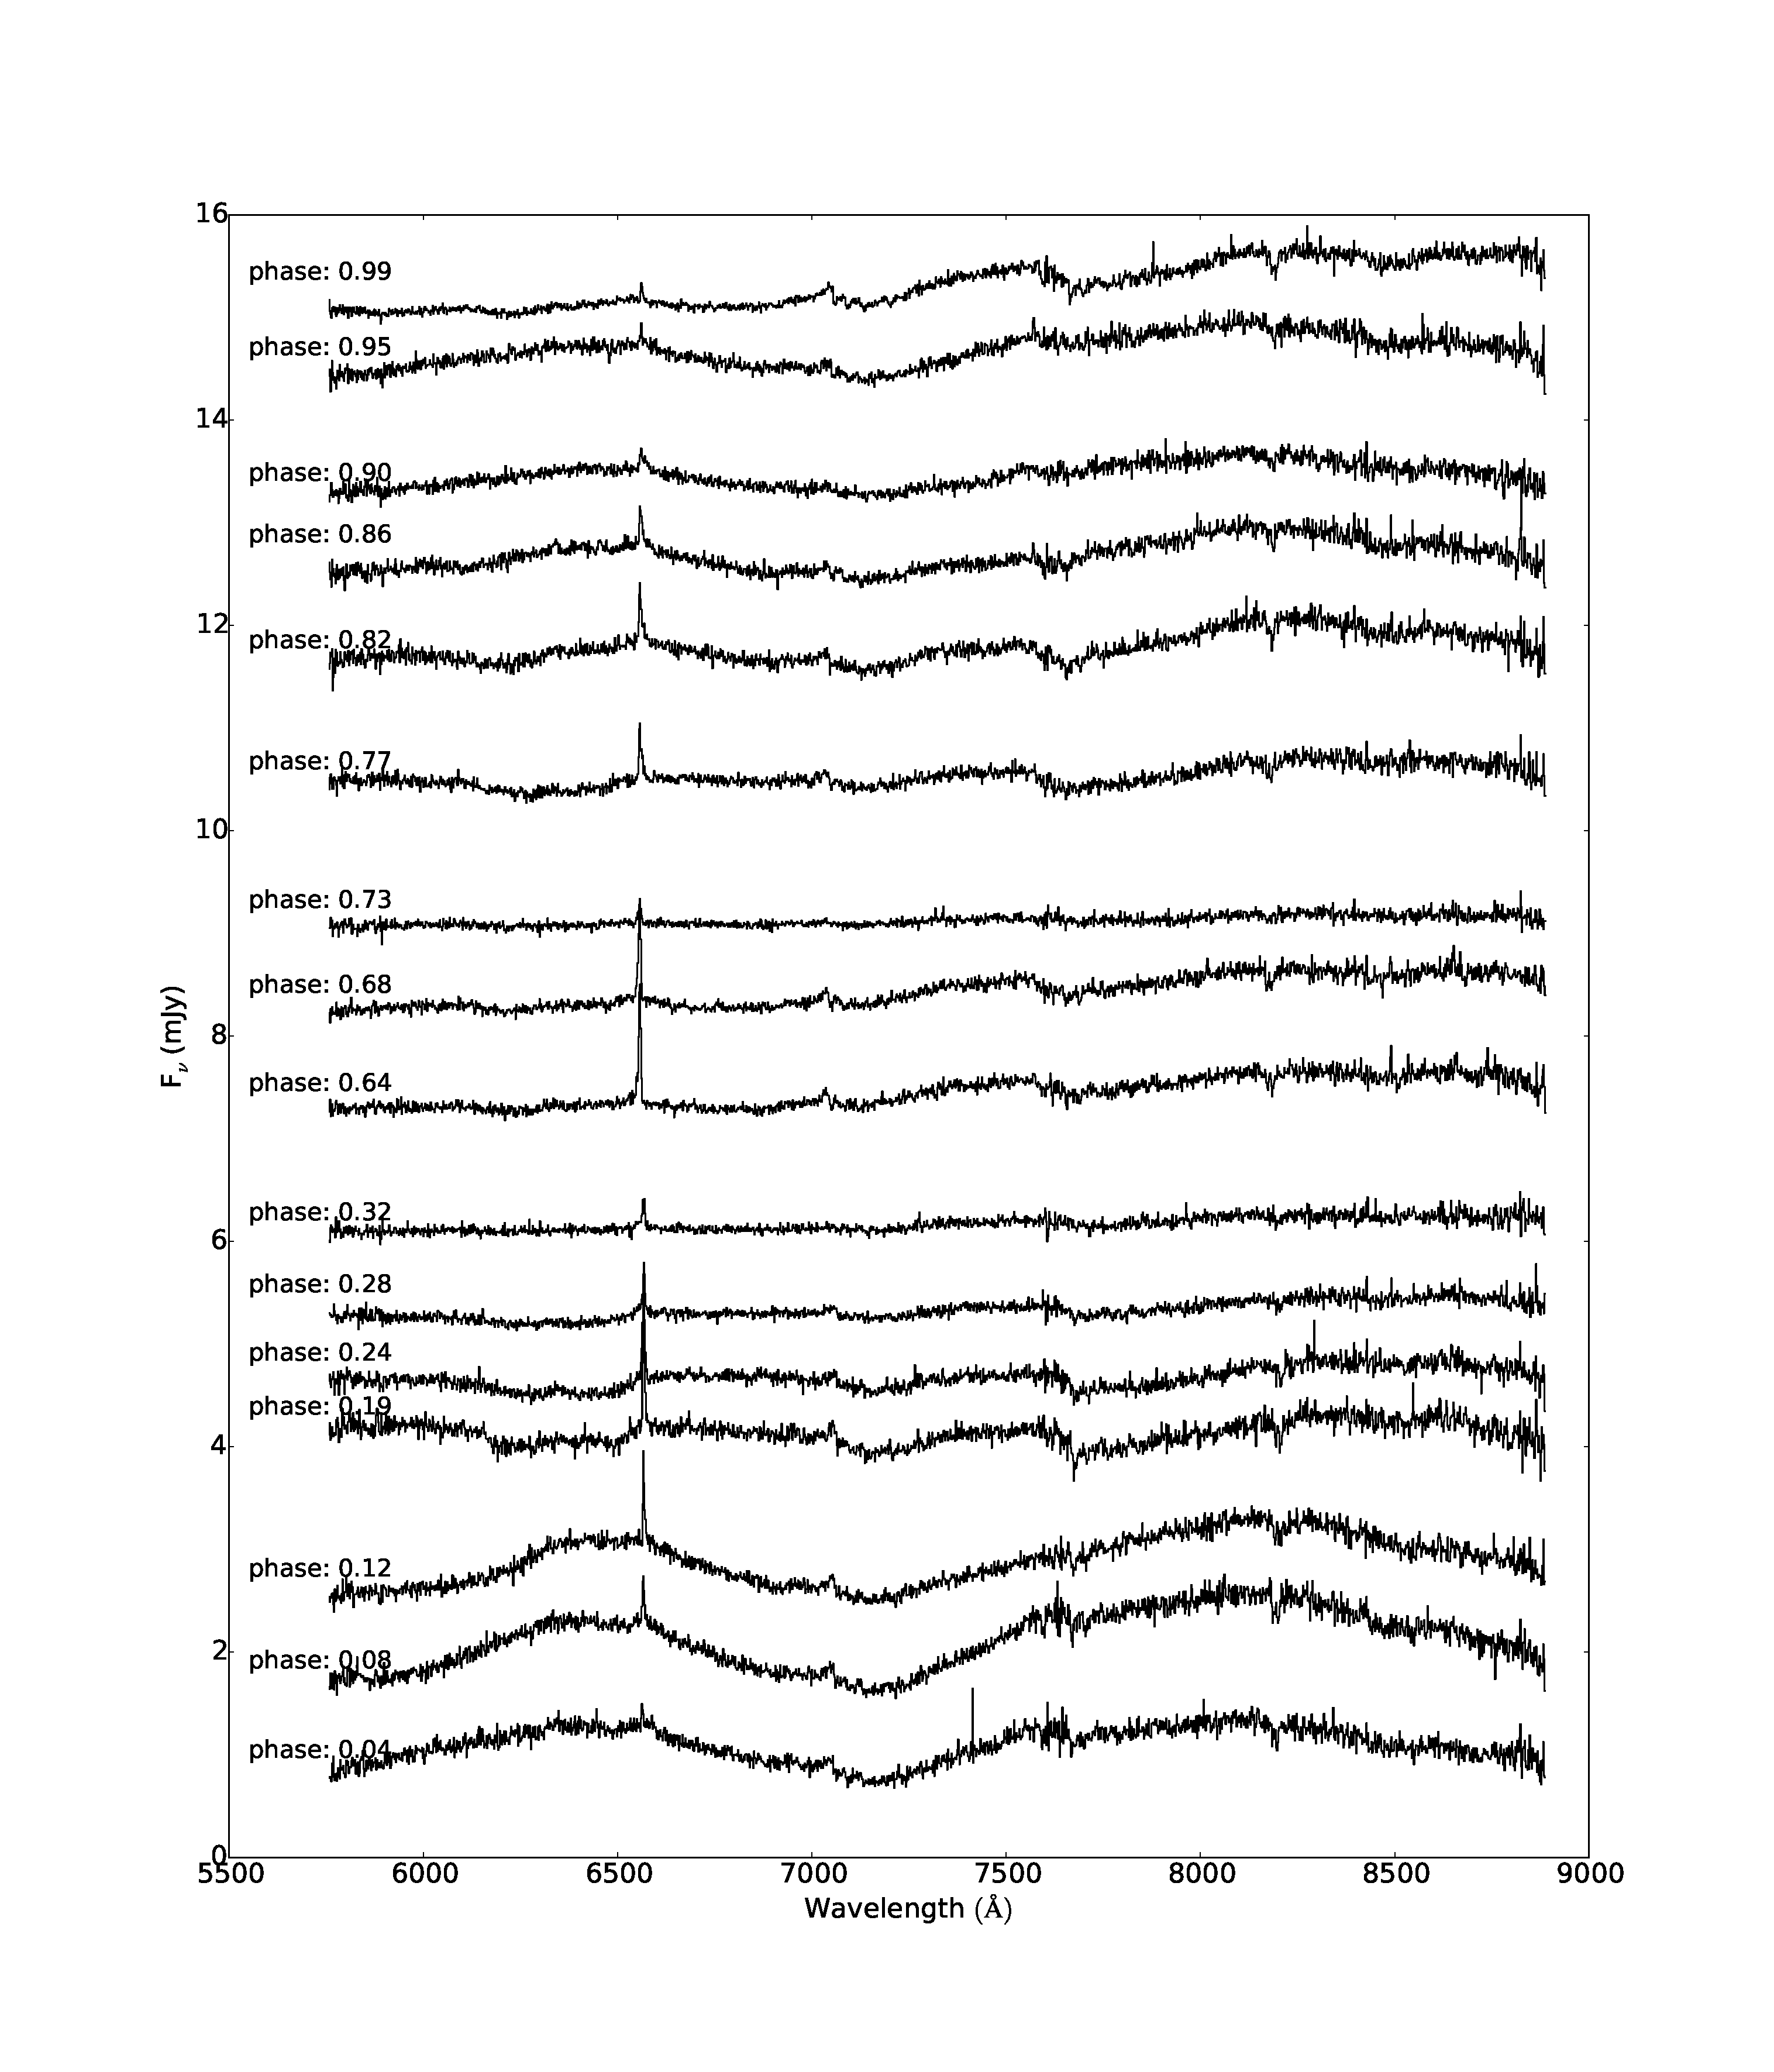
\includegraphics[width=\textwidth]{images/CSS081231_spectra_q.eps}
\caption[Caption for spectra]{The optical spectra of CSS081231 taken at 16 stages of the orbital cycle during quiesence in February 2009.  }
\label{fig:spectra-quiescent}
\end{figure*}

% Quiescent spectra - blue
\begin{figure*}
\centering
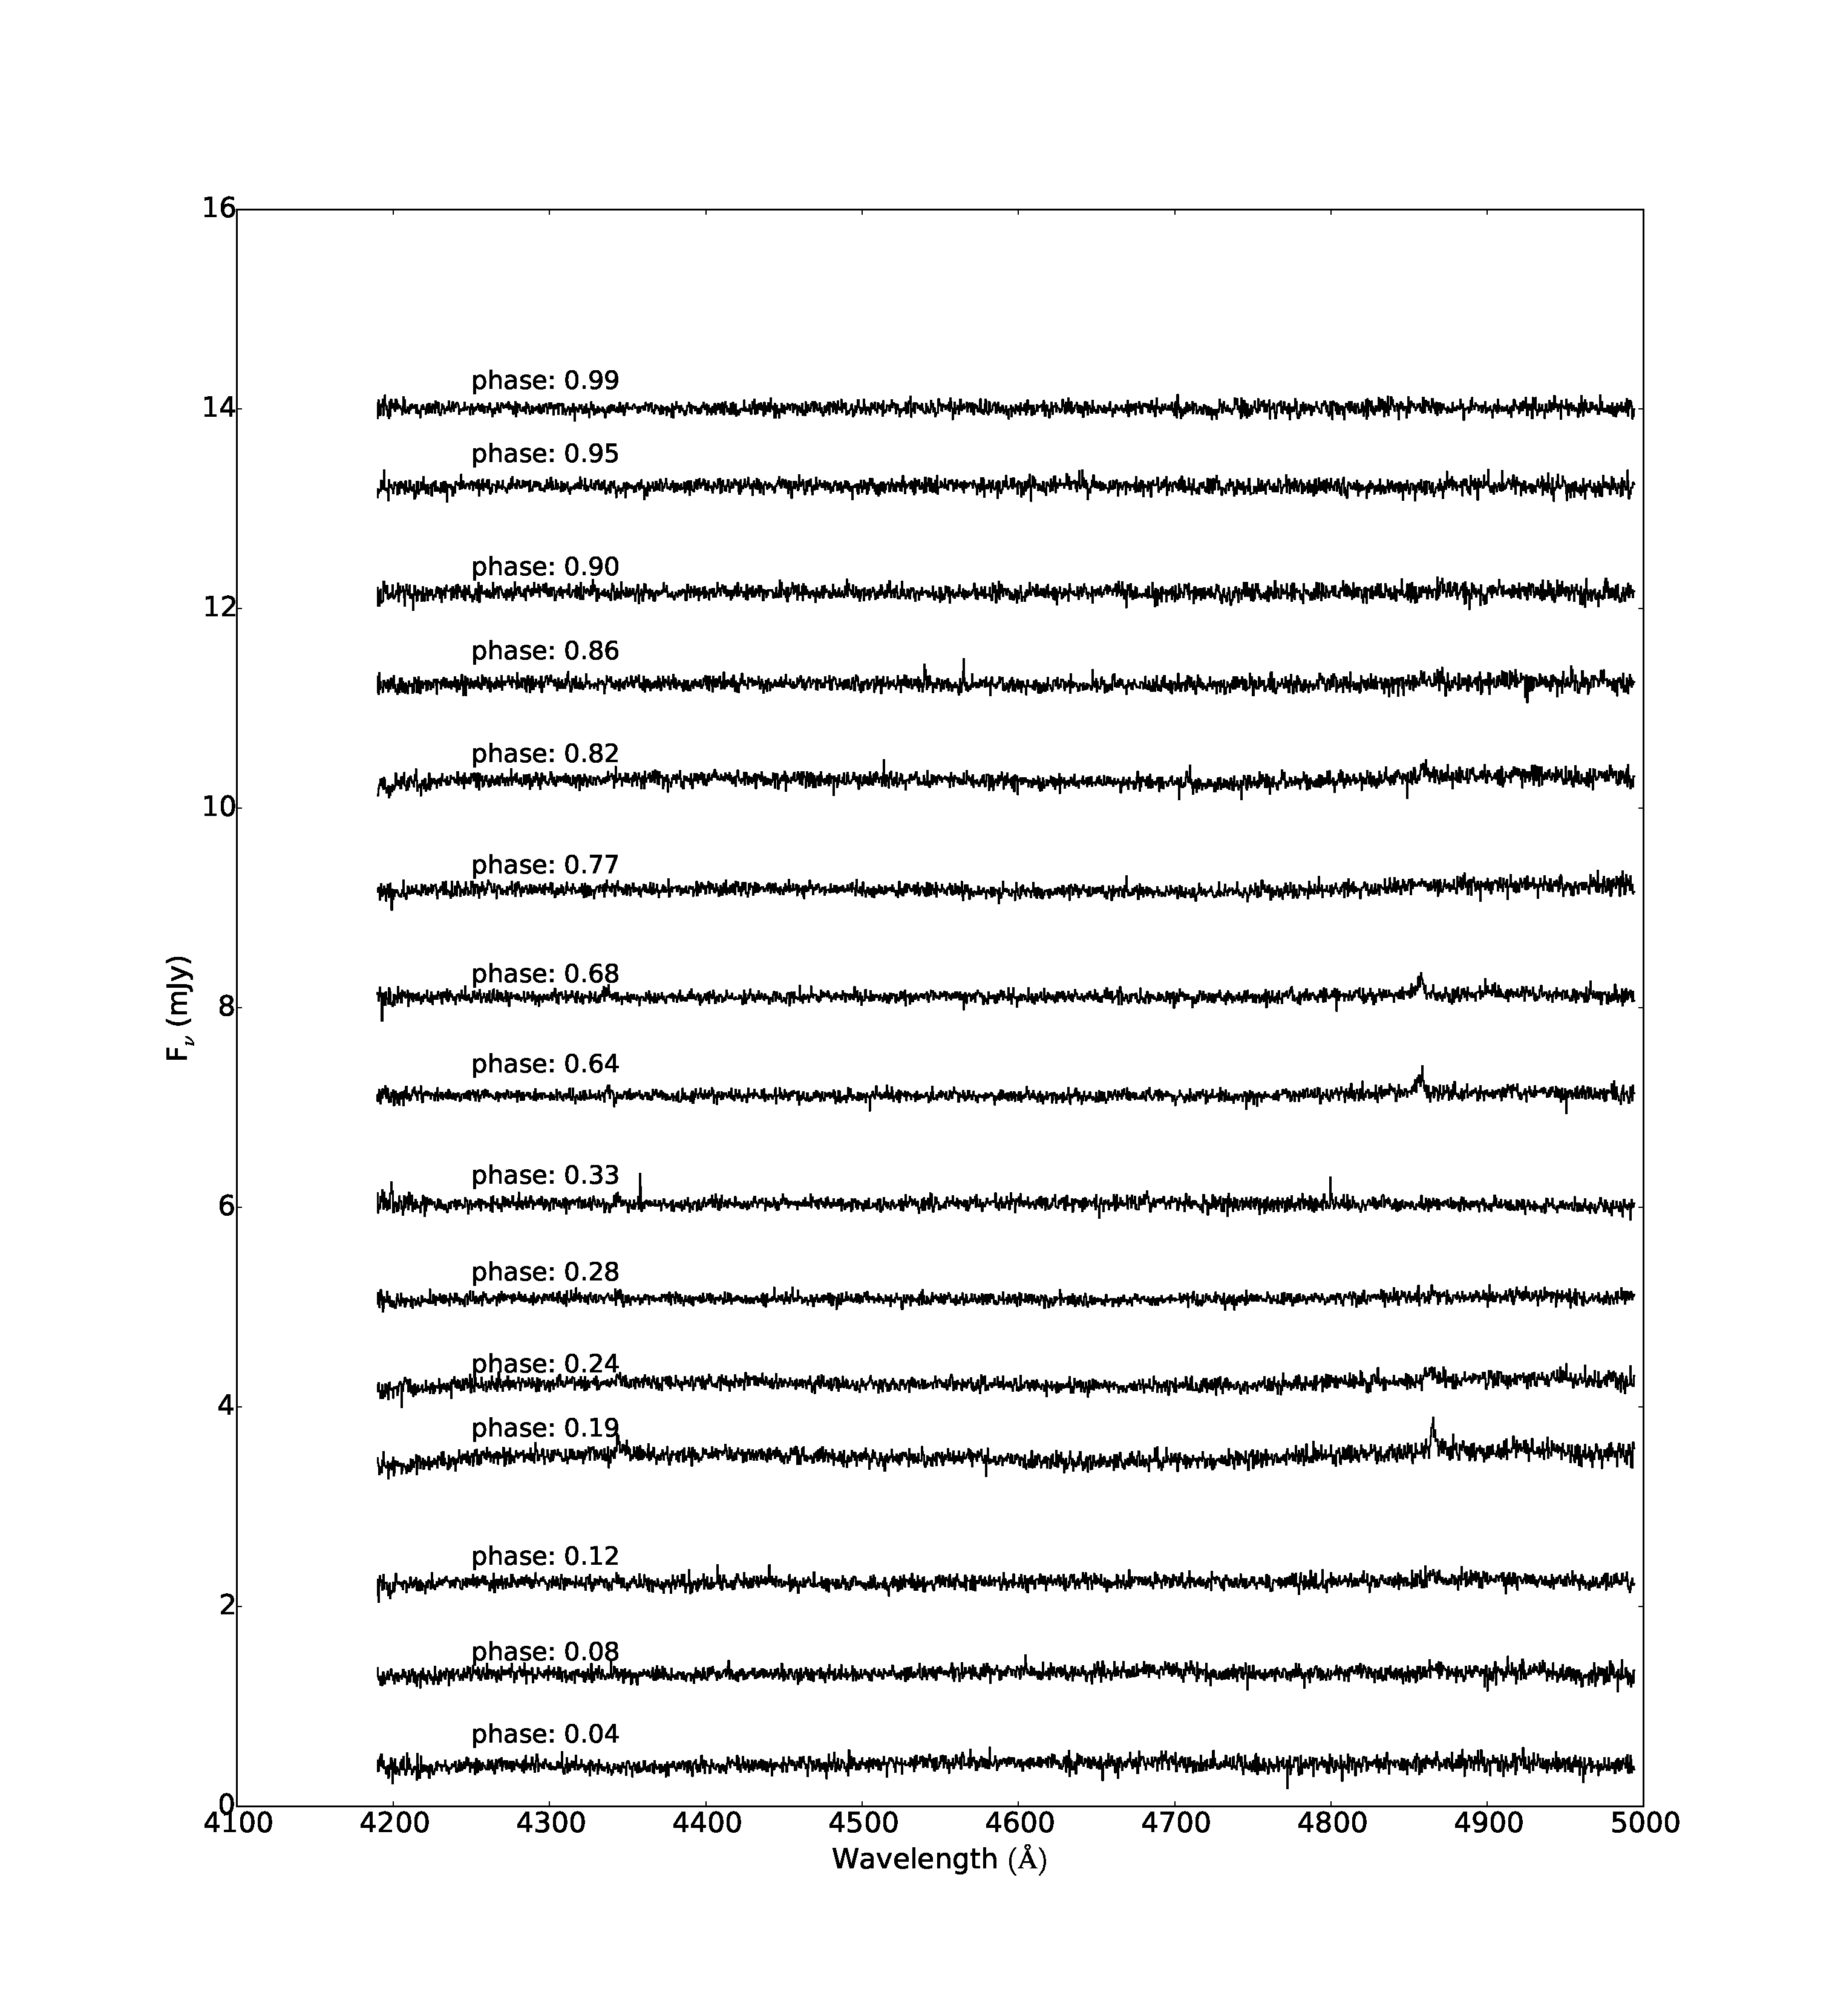
\includegraphics[width=\textwidth]{images/blue_spectra.eps}
\caption[Caption for spectra]{The blue optical spectra of CSS081231 taken at 16 stages of the orbital cycle during quiesence in February 2009.  }
\label{fig:spectra-quiescent}
\end{figure*}

\subsection{Maths}
\label{sec:maths} % used for referring to this section from elsewhere

Simple mathematics can be inserted into the flow of the text e.g. $2\times3=6$
or $v=220$\,km\,s$^{-1}$, but more complicated expressions should be entered
as a numbered equation:

\begin{equation}
    x=\frac{-b\pm\sqrt{b^2-4ac}}{2a}.
	\label{eq:quadratic}
\end{equation}

Refer back to them as e.g. equation~(\ref{eq:quadratic}).

\subsection{Figures and tables}

Figures and tables should be placed at logical positions in the text. Don't worry about the exact layout, which will be handled by the publishers.

Figures are referred to as e.g. Fig.~\ref{fig:example_figure}, and tables as
e.g. Table~\ref{tab:example_table}.


% Example table
\begin{table}
	\centering
	\caption{This is an example table. Captions appear above each table.
	Remember to define the quantities, symbols and units used.}
	\label{tab:example_table}
	\begin{tabular}{lccr} % four columns, alignment for each
		\hline
		A & B & C & D\\
		\hline
		1 & 2 & 3 & 4\\
		2 & 4 & 6 & 8\\
		3 & 5 & 7 & 9\\
		\hline
	\end{tabular}
\end{table}


\section{Conclusions}

The last numbered section should briefly summarise what has been done, and describe
the final conclusions which the authors draw from their work.

\section*{Acknowledgements}

The Acknowledgements section is not numbered. Here you can thank helpful
colleagues, acknowledge funding agencies, telescopes and facilities used etc.
Try to keep it short.

%%%%%%%%%%%%%%%%%%%%%%%%%%%%%%%%%%%%%%%%%%%%%%%%%%

%%%%%%%%%%%%%%%%%%%% REFERENCES %%%%%%%%%%%%%%%%%%

% The best way to enter references is to use BibTeX:

\bibliographystyle{mnras}
\bibliography{../rashley} % if your bibtex file is called example.bib


% Alternatively you could enter them by hand, like this:
% This method is tedious and prone to error if you have lots of references
%\begin{thebibliography}{99}
%\bibitem[\protect\citeauthoryear{Author}{2012}]{Author2012}
%Author A.~N., 2013, Journal of Improbable Astronomy, 1, 1
%\bibitem[\protect\citeauthoryear{Others}{2013}]{Others2013}
%Others S., 2012, Journal of Interesting Stuff, 17, 198
%\end{thebibliography}

%%%%%%%%%%%%%%%%%%%%%%%%%%%%%%%%%%%%%%%%%%%%%%%%%%

%%%%%%%%%%%%%%%%% APPENDICES %%%%%%%%%%%%%%%%%%%%%

\appendix

\section{Some extra material}

If you want to present additional material which would interrupt the flow of the main paper,
it can be placed in an Appendix which appears after the list of references.

%%%%%%%%%%%%%%%%%%%%%%%%%%%%%%%%%%%%%%%%%%%%%%%%%%


% Don't change these lines
\bsp	% typesetting comment
\label{lastpage}
\end{document}

% End of mnras_template.tex